\documentclass[UTF8]{ctexart}
\usepackage[paper=a4paper,dvips,top=2.5cm,left=2.8cm,right=2.8cm,foot=1cm,bottom=3.2cm]{geometry}
\usepackage{fancyhdr}
\usepackage{indentfirst}
\usepackage{enumerate}
\usepackage{clrscode}
\usepackage{listings}
\usepackage{amsmath}
\usepackage{amstext}
\lstset{language=Matlab}%代码语言使用的是matlab
\lstset{breaklines}%自动将长的代码行换行排版
\lstset{extendedchars=false}%解决代码跨页时,章节标题,页眉等汉字不显示的问题
\usepackage{graphicx}
\usepackage[colorlinks,linkcolor=blue,urlcolor = blue]{hyperref}
\DeclareGraphicsExtensions{.eps,.ps,.jpg,.bmp}
\pagestyle{plain}
\begin{document}
\par 尊敬的吴老师,您好
\newline
\par 由于前段时间有个课程大作业,所以阅读论文的进度慢了些。
\par 关于“Learning User-Specific Latent Influence and
Susceptibility from Information Cascades”这篇论文,我前后读了好几遍,并对公式部分结合自己的理解做了翻译。目前对文章所描述的学习过程有了大致的理解,但有些细节还拿不准。比如如何得到$\delta(u,v)$:文章所说的“cascade of message”我暂称为转发链$C^{m}$,“cascade context”为上下文链$D_{v,i}^{m}$。$C^{m}$是针对某条消息的转发用户列表,按转发时间先后排序;$D_{v,i}^{m}$对用户$v$而言是一个随时间不断扩大的用户列表,如图1所示。$\delta(u,v)$表示$u$的消息是否会到达$v$。
\begin{figure}[h!]
    \centering
    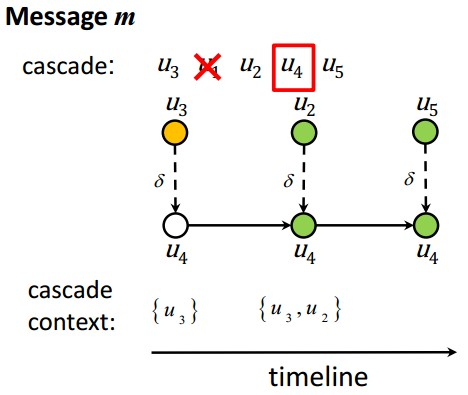
\includegraphics[width=8cm]{0507-1.jpg}
    \caption{LIS model}
    \label{fig-sample}
\end{figure}
\par 文章中提到$\delta(u,v)$是这样得到的:“the aggregate diffusion network of historical cascades
of messages”,更具体一点的解释是这样的:“we estimate diffusion network according
to a large collection of historical cascades: one cascade has
a collection of forwarding traces over the period of observation, forming a directed graph. We aggregate these graphs
of all cascades into a diffusion network”。为了方便理解,作者还给了配图2。diffusion network包括LIS model、social influence和cascade context的叠加。
\begin{figure}[h!]
    \centering
    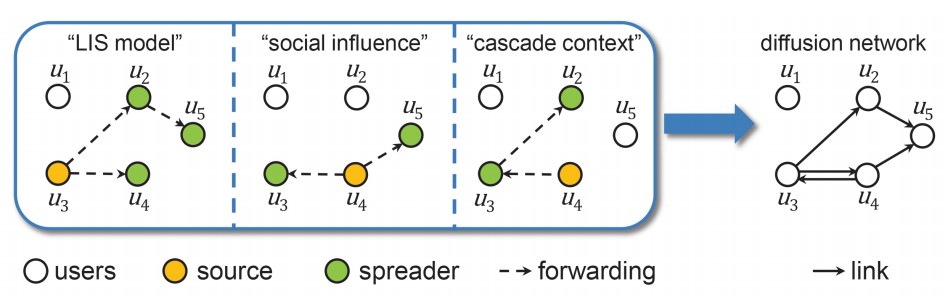
\includegraphics[width=10cm]{0507-2.jpg}
    \caption{各种“链”叠加构成网络}
    \label{fig-sample}
\end{figure}
\par在这里我有疑问,假如是微博网络的话,social influence应该是关注或被关注关系;cascade context是随时间变化的,而$\delta(u,v)$与时间无关,应该怎么取cascade context?另外对这里的LIS model的具体意义也不清楚。
\par 关于文章所用数据集,包括人为合成数据集和现实网络数据集。人为合成数据集有两个:1000节点的BA网络和随机网络,现实网络数据集来自于WISE 2012 Challenge,是一份从2011年1月1号到2011年2月15号微博数据。官网\href{http://www.wise2012.cs.ucy.ac.cy/challenge.html}{WISE}提供的数据集链接均已失效,我用google也没能找到,该怎么办?
\end{document}
